%\documentclass[aps,prstab,showpac,twocolumn]{revtex4-1}  
%\documentclass[aps,prstab,onecolumn,preprint]{revtex4-1}
\documentclass[aps,prstab,onecolumn,preprint,endfloats]{revtex4-1}

\usepackage{graphicx}
\usepackage{epsfig}
\usepackage{subfigure}
\usepackage{fancyhdr}
\usepackage{color}
\usepackage{amsfonts}
\usepackage{amsmath}
\usepackage{amssymb}
\usepackage{dcolumn}
\usepackage{bm}
\usepackage{indentfirst}
\usepackage{rotating}
\usepackage{moreverb}

\setlength{\textwidth}{6.5in}
\setlength{\textheight}{8.5in}
\setlength{\topmargin}{0in}
\setlength{\oddsidemargin}{0.0in}
\setlength{\evensidemargin}{0.0in}
\setlength{\rightmargin}{0.0in}

\linespread{0.956}

\makeatletter

\begin{document}

\title{Studies of Particle Motions During Slow Resonant Extraction}
\author{Chong Shik Park, James Amundson, Leo Michelotti, and Vladimir Nagaslaev}
\affiliation{Fermi National Accelerator Laboratory, PO Box 500, Batavia, IL 60510}
\date{\today}

\begin{abstract}
We present here 
%The Mu2e experiment at Fermilab requires the acceleration and transport of intense proton beams, and the delivery of stable and uniform particle spills to the production target. To meet the experimental requirement, particles will be slowly extracted from the Delivery Ring to the external beamline. Using Synergia2, we have performed multi-particle tracking simulations of the third-integer resonant extraction in the Delivery Ring, including space charge effects as well as physical beamline elements and apertures. With a suitable ramp profile of tune-quadrupoles, we modeled a uniform spill structure. In order to minimize beam losses which are critical for efficient extractions, we have implemented a number of features, such as apertures in beamline elements, septum plane alignments. The RF Knockout (RFKO) technique, which excites particles transversely, is employed as a spill regulation system. Combined with a feedback system, it assists in fine-tuning the spill uniformity. Simulation studies have been carried out to optimize the RFKO feedback scheme, which will be helpful in designing the spill regulation system. 
\end{abstract}

\pacs{}
\maketitle

\setcounter{tocdepth}{5}

%\tableofcontents

%%%%%%%%%%%%%%%%%%%%%%%%%%%%%%%%%%%%%%%%%%%%%%%%%%%%%%%%%%%%%%%%%%%%%%
\section{\label{sec:intro}Introduction}

\clearpage

\section{\label{sec:bump}Local Orbit Corrections with Dynamic Bumps}

In the previous paper~\cite{mu2e}, we discussed that a septum foil plane should be aligned with particles' entrance angles to the septum because of its finite length.
This alignment of the septum foil plane should be optimized in the manner of reducing particle losses due to crossing the plane from outside to inside the field region or vice versa.
In the Delivery Ring, however, the septum is placed at a zero dispersion section, and all shrinking separatrices are always centered at origin during an entire extraction period.
These yield that the Hardt condition, a condition to arrange separatrix geometries by superimposing them for different momenta, cannot be fullfiled.
Consequently, particles' angle coordinates at the entrance of the first septum are varying in time.

\begin{figure*}[!htbp]
  \subfigure[Before applying dynamic bumps]{
    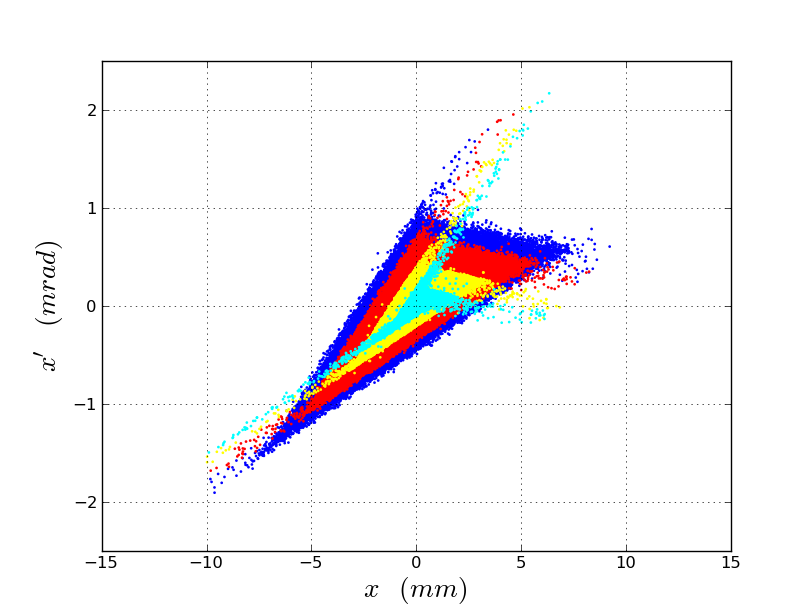
\includegraphics[width=.45\textwidth]{img/bump40.png}
    \label{fig:bump00}}
  \subfigure[After applying dynamic bumps]{
    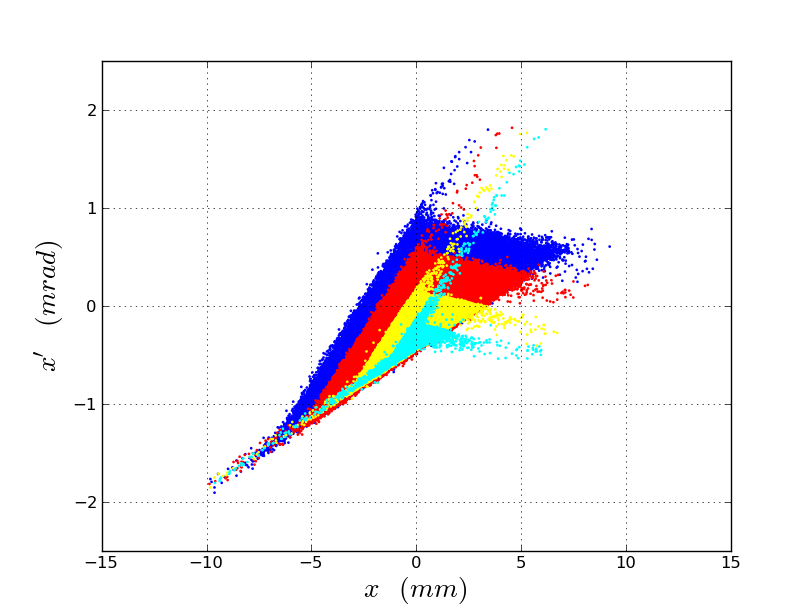
\includegraphics[width=.45\textwidth]{img/bump41.png}
    \label{fig:bump01}}
  \caption{\label{fig:bump0}Phase space plots of particles for 4 different extraction stages (100, 10000, 20000, 30000 turns): (a) before and (b) after applying dynamic bump corrections}
\end{figure*}

Fig.~\ref{fig:bump00} shows a phase space of particles for 4 different extraction stages.
As the separatrix is squeezed by increasing tune-quad strengths, unstable particles are streamed along branches of separatrices. 
The septum field region is formed on the [left] side of the vertical line (color: purple) at $x=10$ mm. 
The gray shadows on the plot are defined as the septum shadow regions in which particles will be considered as lost~\cite{m.pullia}.
Streams of unstable particles on the [leftmost] separatrix branch for each stage are entering the septum field region by crossing the septum foil line.
However, their entering angles are moving [upward] during the extraction processes.
An angle of the septum foil plane is aligned with an initial extraction stage.
Therefore, the alignment is only valid for few turns at the beginning, and there will be continuous misalignments of the septum foil plane later.
These result that more particles are entering the [upper] septum shadow region (color:gray shadow), and they will be lost.
Variations of angle coordinates at the septum entrance will eventually be seen at the experiment target with large horizontal angular spread of extracted beams.

In our case with a zero dispersion at the setum, there are two possible ways to have same entrance angle of the beam to the septum for different extraction stages.
One method is to compesnate the beam angle by rotating the separatrix. This could be achievable by changing phases of two harmonic sextupole circuits.
The phase contributions of each harmonic circuit differs by about 90 deg, and these make phase adjusments doable.
However, particles' entrance angles for different extraction stages are same only if their $x$ coordinates are equal to the horizontal position of the septum foil at the entrance, $x_{ES}$.
In other words, their angles beyond $x_{ES}$ will be diverged.
These results in an asymmetric angular spread of extracted beams.
The other solution is to apply local orbit corrections using dynamic angle bumps throughout the spill.
With this method, extracted particles will have a symmetric angluar spread during the spill.
For resonant extraction from the Delivery ring, we choose the dynamic bump scheme.
As an alternative backup solution to prepare a failure of local bump corrections, the harmonics sextupole magnets and their power supplies are designed to preserve ramp capabilities.
In this paper, we will only discuss how local bump corrections are implemented.

\begin{figure}[!htbp]
  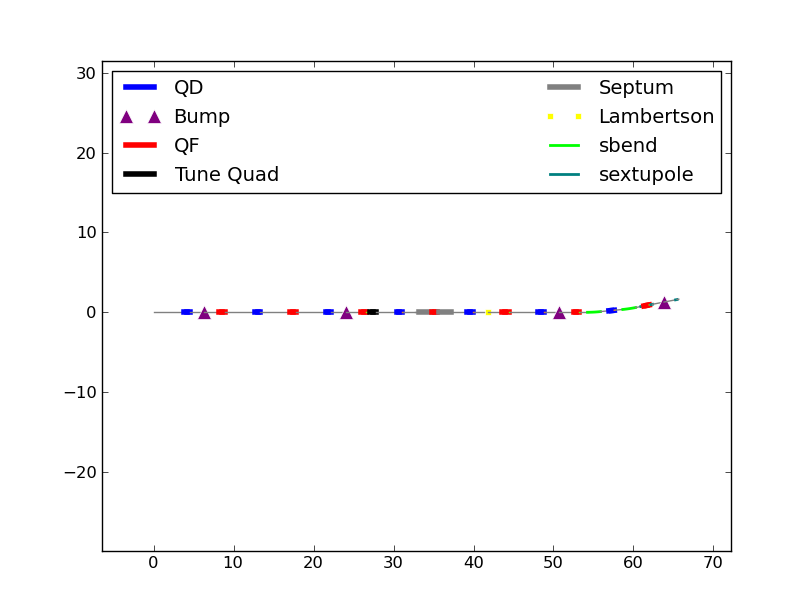
\includegraphics[width=.45\textwidth]{img/20140109-00.png}
  \caption{\label{fig:bump1}Schematic drawing of the external beamline with 4 local orbit bumps.}
\end{figure}

Using 4 dynamic bumps, we could align separatrices to reduce anglular deviations at the entrance of the septum.
Fig.~\ref{fig:bump1} shows a schematic drawing of 4 dynamic bump locations in the extraction beamline.
2 bumps are located at the upstream of septa, and the other 2 are at the downstream.
Upstream bumps kick particles so that the base of separatirces are aligned during the entire extraction period.
Then, downstream bumps will kick them back to original orbits.
Fig.~\ref{fig:bump01} shows a phase space plot of particles for different extraction stages after applying local orbit corrections.
All trainglular distrbutions of particles are well aligned on theire bases.
The [leftmost] branch arms are extended to the same direction, i.e., particles are entering the septum field region with the same angle.

Strengths of local orbit corrections can be easily obtained by applying the transfer matrix method with initial closed orbit conditions.
Using the condition that the closed orbit is zero outside bumps, their strengths in time, $\theta_{i}(t)$ for $i=1,2,3,4$, are given by
\begin{equation}
  \begin{split}
  \theta_{1}(t) & = \sqrt{\frac{\beta_{s}}{\beta_{1}}}
               \frac{\sin(\psi_{s} - \psi_{2})}
                    {\sin(\psi_{2} - \psi_{1})}
               \left( - \Delta x_{s}^{\prime} (t) \right),
  \\ %\;\;\;
  \theta_{2}(t) & = \sqrt{\frac{\beta_{s}}{\beta_{2}}}
               \frac{\sin(\psi_{s} - \psi_{1})}
                    {\sin(\psi_{2} - \psi_{1})}
               \Delta x_{s}^{\prime} (t), \\
  \theta_{3}(t) & = \sqrt{\frac{\beta_{s}}{\beta_{3}}}
               \frac{\sin(\psi_{s} - \psi_{4})}
                    {\sin(\psi_{4} - \psi_{3})}
               \Delta x_{s}^{\prime} (t),
  \\ %\;\;\;\;\;\;\;\;\;\;
  \theta_{4}(t) & = \sqrt{\frac{\beta_{s}}{\beta_{4}}}
               \frac{\sin(\psi_{s} - \psi_{3})}
                    {\sin(\psi_{4} - \psi_{3})}
               \left( - \Delta x_{s}^{\prime} (t) \right),
  \end{split}
\end{equation}
where $\beta_{i}$'s are betatron functions at the septum($s$) and bumps($1,2,3,4$), $\psi_{i}$'s are betatron phase advances, and $\Delta x^{\prime}_{s} (t)$ is the required angle kicks of particles at the septum entrance as a function of time.
Fig.~\ref{fig:bump2} shows changes of bump strengths vs.~time.
Since particles' entrance angles to the septum are aligned to the initial extraction stage, bump strengths are zero at the beginning and are maximum at the end of extraction.

\begin{figure}[!htbp]
  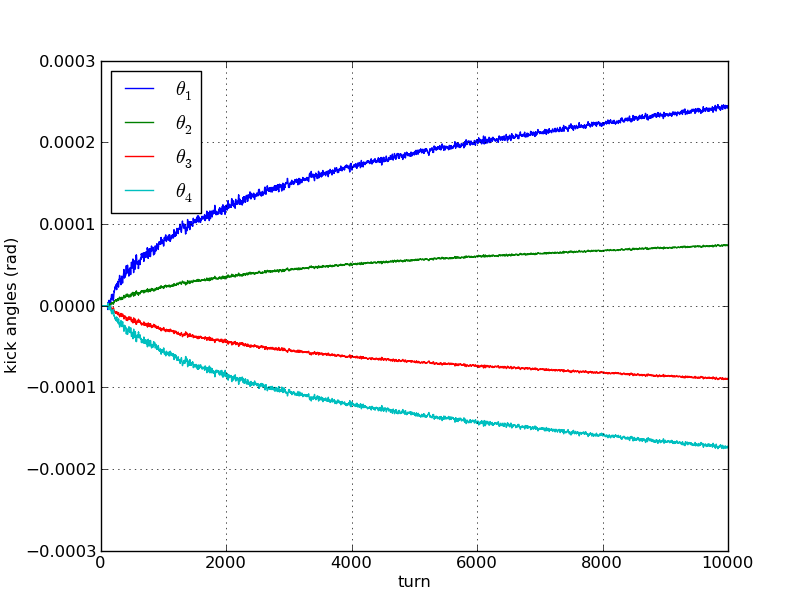
\includegraphics[width=.45\textwidth]{img/20140123-00.png}
  \caption{\label{fig:bump2}Strengths changes of dynamic bumps in time.}
\end{figure}

\begin{figure*}[!htbp]
  \subfigure[Before applying dynamic bumps]{
    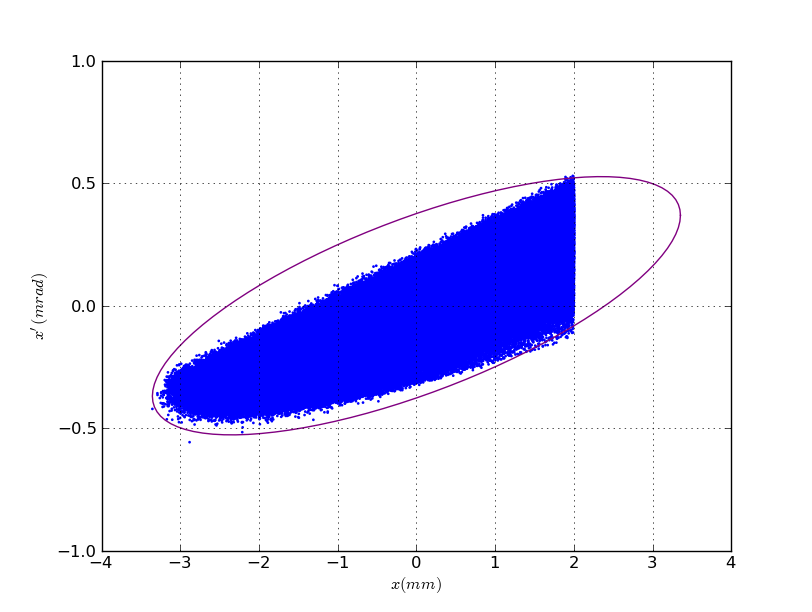
\includegraphics[width=.45\textwidth]{img/20140206-02.png}
    \label{fig:bump30}}
  \subfigure[After applying dynamic bumps]{
    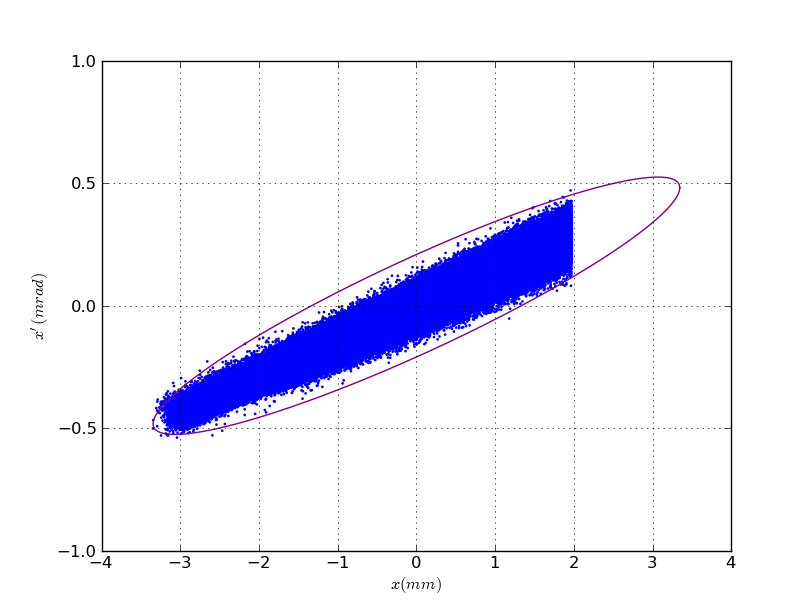
\includegraphics[width=.45\textwidth]{img/20140206-03.png}
    \label{fig:bump31}}
  \caption{\label{fig:bump3}Footprints of extracted particles with/without dynamic bumps.}
\end{figure*}

\begin{figure}[!htbp]
  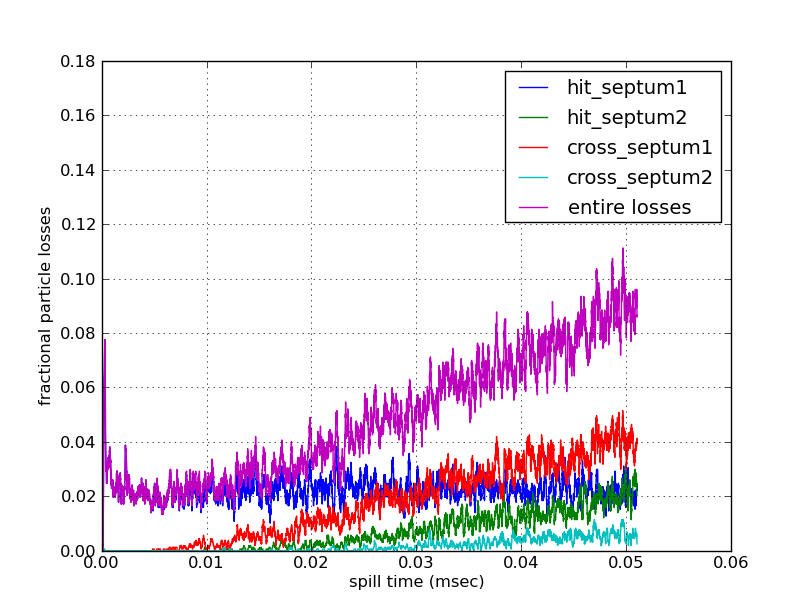
\includegraphics[width=.45\textwidth]{img/20140203-06.png}
  \caption{\label{fig:bump4}Particle losses in time with/without dynamic bumps.}
\end{figure}

\clearpage

\section{\label{sec:loss}Tracking of Particle Losses}

\section{\label{sec:arrival}Arrival Time Distribution}

\section{\label{sec:rfko}RFKO Beam Distribution Function}

\section{\label{sec:emit}Emittance Growth Rates with RFKO Beam Heating}

\section{\label{sec:conclusion}Conclusion}

\section{\label{thanks}Acknowledgments}

\begin{thebibliography}{77}

  \bibitem{mu2e}
  C.S. Park, ``Tracking Simulation of the Third-Integer Resonant Extraction for the Fermilab Mu2e Experiment,'' submitted to PRST-AB.

  \bibitem{m.pullia}
  M. Pullia, thesis

\end{thebibliography}

\clearpage

\end{document}

%sagemathcloud={"zoom_width":100}